\subsection{Exercise 4a}
 Follow Euler Mehtod, we have:\\
\indent $CO_{2Air(thEx4a)}=CO_{2Air}+CO_{2AirRate}*h$\\
\indent $CO_{2Top(thEx4a)}=CO_{2Top}+CO_{2TopRate}*h$
 Follow order 4 Runge-Kutta method, we have:\\
\indent $k_{1}=f(tn,xn)$;\\
\indent $k_{2}=f(tn+0.5*h,xn+0.5*h*k_{2})$;\\
\indent $k_{3}=f(tn+0.5*h,xn+0.5*h*k_{2})$;\\
\indent $k_{4}=f(tn+h,xn+0.5*h*k_{3})$;\\
\indent $xn+1=xn+(\frac{1}{6})*h*(k_{1}+2k_{2}+2k_{3}+k_{4})$;\\
 However, as we tested the derivatives of $CO_{2AirTop}$ over the derivatives of time are constant so that: $k_{1}=k_{2}=k_{3}=k_{4}=CO_{2AirTopRate}$. We have:\\
\indent $CO_{2AirTop(t+h)}=CO_{2AirTop}+(\frac{1}{6})*h*(6*CO_{2AirTopRate})$\\
 Where,\\
$CO_{2Air(thEx4a)}$ is $CO_{2Air}$ at $t+h$;\\
$CO_{2Top(thEx4a)}$ is $CO_{2Top}$ at $t+h$;\\
$CO_{2AirTop(t+h)}$ is $CO_{AirTop}$ at $t+h$;\\
$CO_{2Air}$ is $CO_{2Air}$ concentration at $t$;\\
$CO_{2Top}$ is $CO_{2Top}$ concentration at $t$;\\
$CO_{2AirTop}$ is $CO_{2AirTop}$ concentration at $t$;\\
$CO_{2AirRate}$ is rate change of $CO_{2Air}$ concentration as derivative of $CO_{2Air}$ over dt;\\
$CO_{2TopRate}$ is rate change of $CO_{2Top}$ concentration as derivative of $CO_{2Top}$ over dt;\\
$CO_{2AirTopRate}$ is rate change of $CO_{2AirTop}$ concentration as derivative of $CO_{2AirTop}$ over dt;\\














\subsection{Exercise 4b}
Using Euler method in exercise 1, (figure 8)
\begin{figure}[h]
    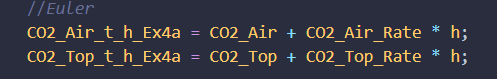
\includegraphics[width = 5.5in, height = 1in]{Code/Pic/ex4_euler.png}
    \caption{Euler Method}
    \label{fig:my_label}
\end{figure}

We already have the CO2\_Air\_Rate and CO2\_Top\_Rate in exercise 2, and h is given in this exercise, thus we already have everything we need to execute the method.

Below is the result of the programm

\begin{figure}[h]
\centering
    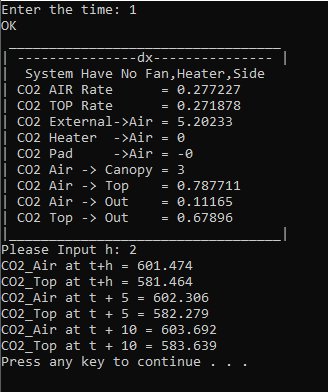
\includegraphics[width = 2.5in, height = 2.5in]{Code/Pic/final1.png}
    \caption{Programm output}
    \label{fig:my_label}
\end{figure}

\begin{figure}[h]
\centering
    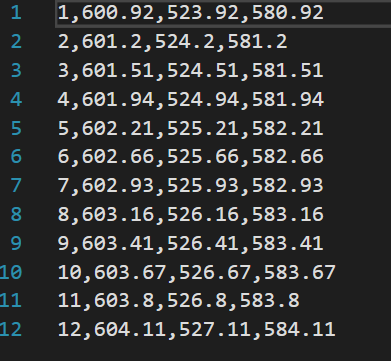
\includegraphics[width = 2in, height = 2.5in]{Code/Pic/final2.png}
    \caption{Measured data}
    \label{fig:my_label}
\end{figure}
\subsection{Conclusion}
By comparing the output with the measured data below, we can see that: 
With $t=1 \longrightarrow t+5=6, t+10=11$
\begin{itemize}
    \item CO2\_Air at 6 min is 602.306, CO2\_Top at 6 min = 582.279
    
    Compare to 
    actual data $CO_2_{Air}$ and $CO_2_{Top}$ being 602.66 and  582.66 at 6 minutes respectively
    \item CO2\_Air at 6 min is 603.692, CO2\_Top at 6 min = 583.639
    
    Compare to 
    actual data $CO_2_{Air}$ and $CO_2_{Top}$ being 603.8 and  583.8 at 6 minutes respectively
\end{itemize}

It is clear that we have a very small margin of error (around 0.02\%). Thus, the programm have a very good accuracy.











